\subsection{Receiver Operating Characteristic Curve}

Before discussing the curve, we'll look at what we evaluate. 
\begin{figure}[H]
  \centering
  \begin{subfigure}{0.9\textwidth}
    \centering
    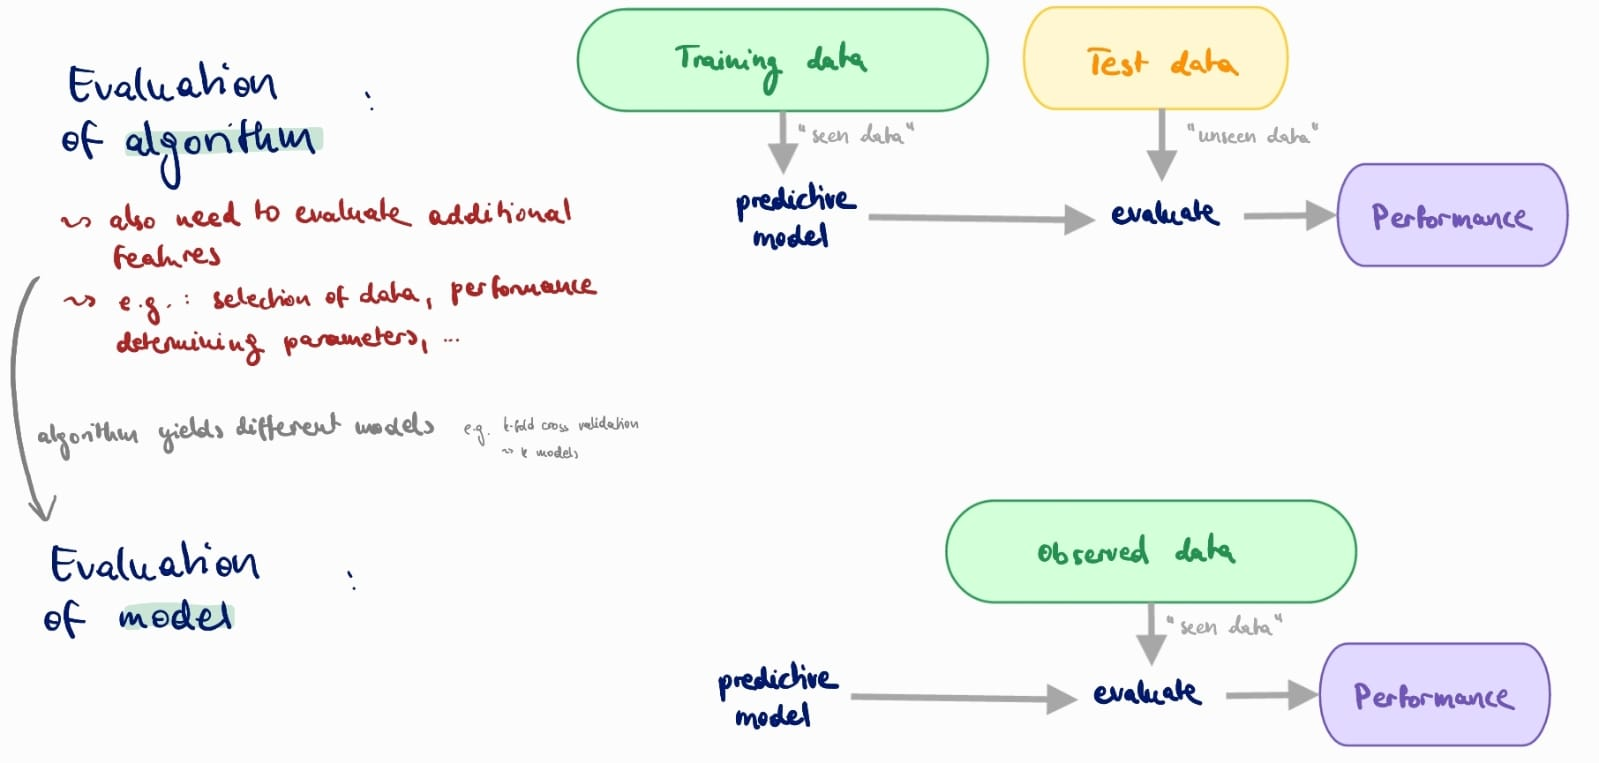
\includegraphics[width=\textwidth]{assets/sl/ct__evaluation.jpg}
  \end{subfigure}

  \caption{What is evaluated?}
  \label{fig:7_rocc_evaluation}
\end{figure}

Now it could happen, that we only have positive observations (common e.g. in process discovery). This can originate from the "survival bias" which describes that positive examples are more likely to be recorded. $FP$ and $TN$ can then of course not be calculated, and the evaluation is just as the training more difficult.

Now, let's move on the the ROCC. Assume we have a non-binary outcome with the resulting value being between $0.0$ and $1.0$, the \textbf{prediction score}\sidenote{Prediction score}.
\begin{itemize}
  \item $0$ means "pretty sure" the predicted class is negative, $1$ means "pretty sure" the predicted class is positive
  \item The question for all in-between values (especially $0.5$): which class are they assigned to, and where to put the threshold?
  \item By playing with the threshold, different confusion matrices are created. 
\end{itemize}

\begin{figure}[H]
  \centering
  \begin{subfigure}{0.7\textwidth}
    \centering
    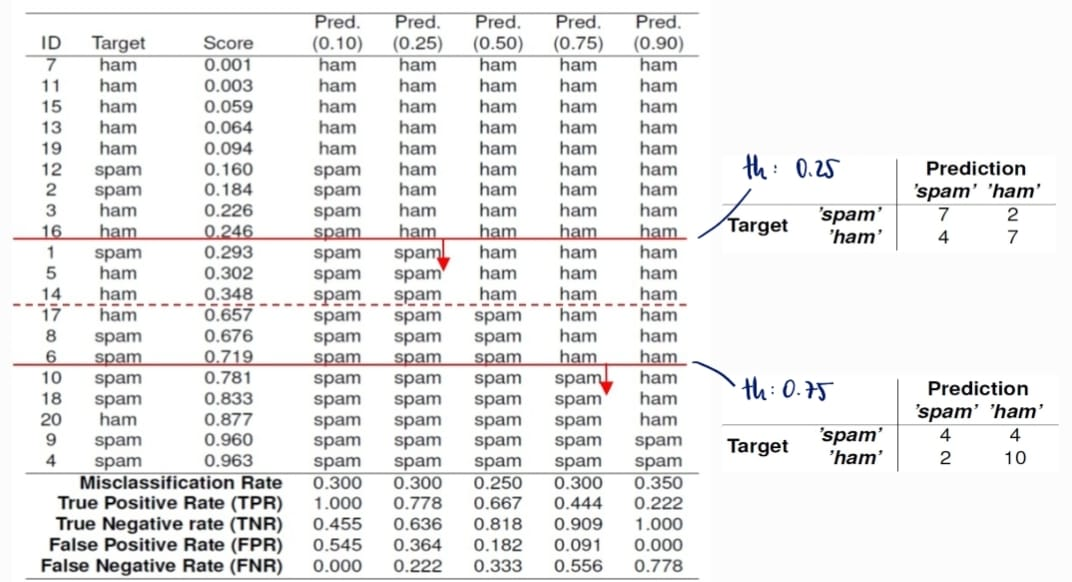
\includegraphics[width=\textwidth]{assets/sl/rocc__playing_threshold.jpg}
  \end{subfigure}

  \caption{Playing with prediction score threshold (and resulting confusion matrix)}
  \label{fig:7_ross_score_th}
\end{figure}

To evaluate which threshold to choose, look at the $TNR$ and $TPR$ as in \ref{fig:7_rocc_tnr_vs_tpr}
\begin{figure}[H]
  \centering
  \begin{subfigure}{0.8\textwidth}
    \centering
    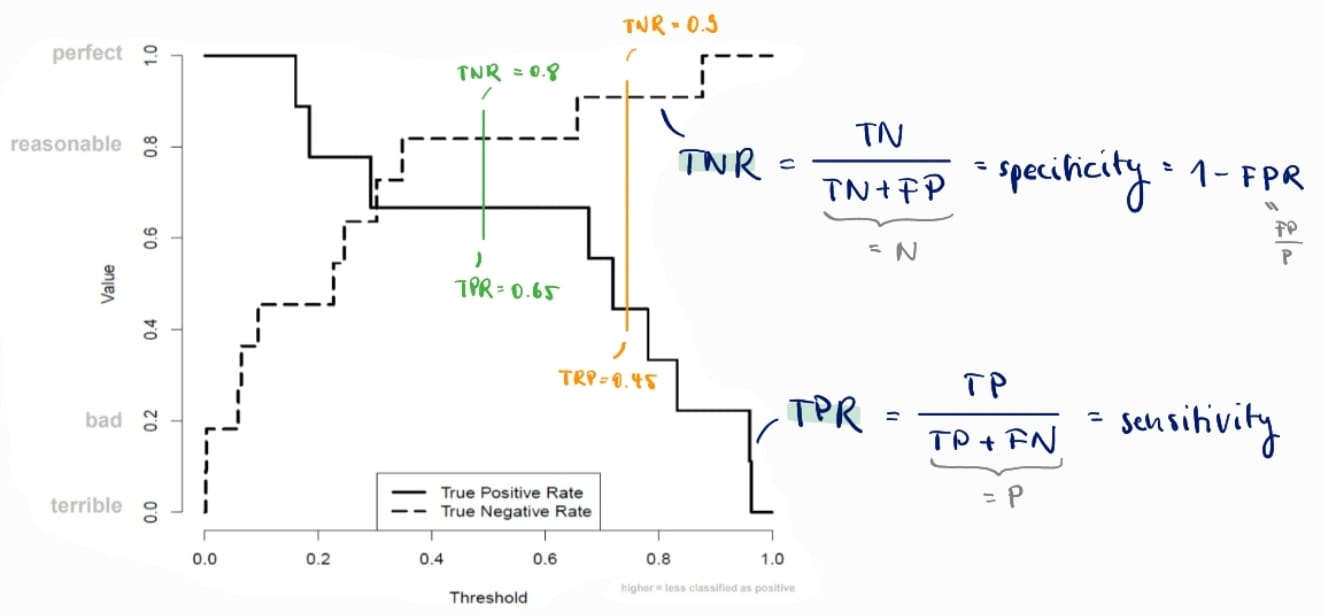
\includegraphics[width=\textwidth]{assets/sl/rocc__treshold_evaluation.png}
  \end{subfigure}

  \vspace*{0.5cm}
  \begin{subfigure}{\textwidth}
    \text{Goal: both $TNR$ and $TPR$ should be as high as possible, but there is a clear trade-off}
    \\

    \begin{subfigure}{0.45\textwidth}
      \begin{itemize}\footnotesize
        \item \text{Sensitivity ($TPR$) as the fraction of positives classified as positive}
      \end{itemize}
    \end{subfigure}
    \vspace*{0.05\textwidth}
    \begin{subfigure}{0.45\textwidth}
      \begin{itemize}\footnotesize
        \item \text{Specificity ($TNR$) as the fraction of negatives classified as negative}
      \end{itemize}
    \end{subfigure}
  \end{subfigure}

  \caption{How to choose prediction score threshold}
  \label{fig:7_rocc_tnr_vs_tpr}
\end{figure}

Using these values, we can now draw a \textbf{receiver operating characteristic} curve\sidenote{Receiver Operating Characteristic Curve}. We have the goal to beat the random guessing line.

\begin{figure}[ht]
  \centering
  \begin{subfigure}{0.4\textwidth}
    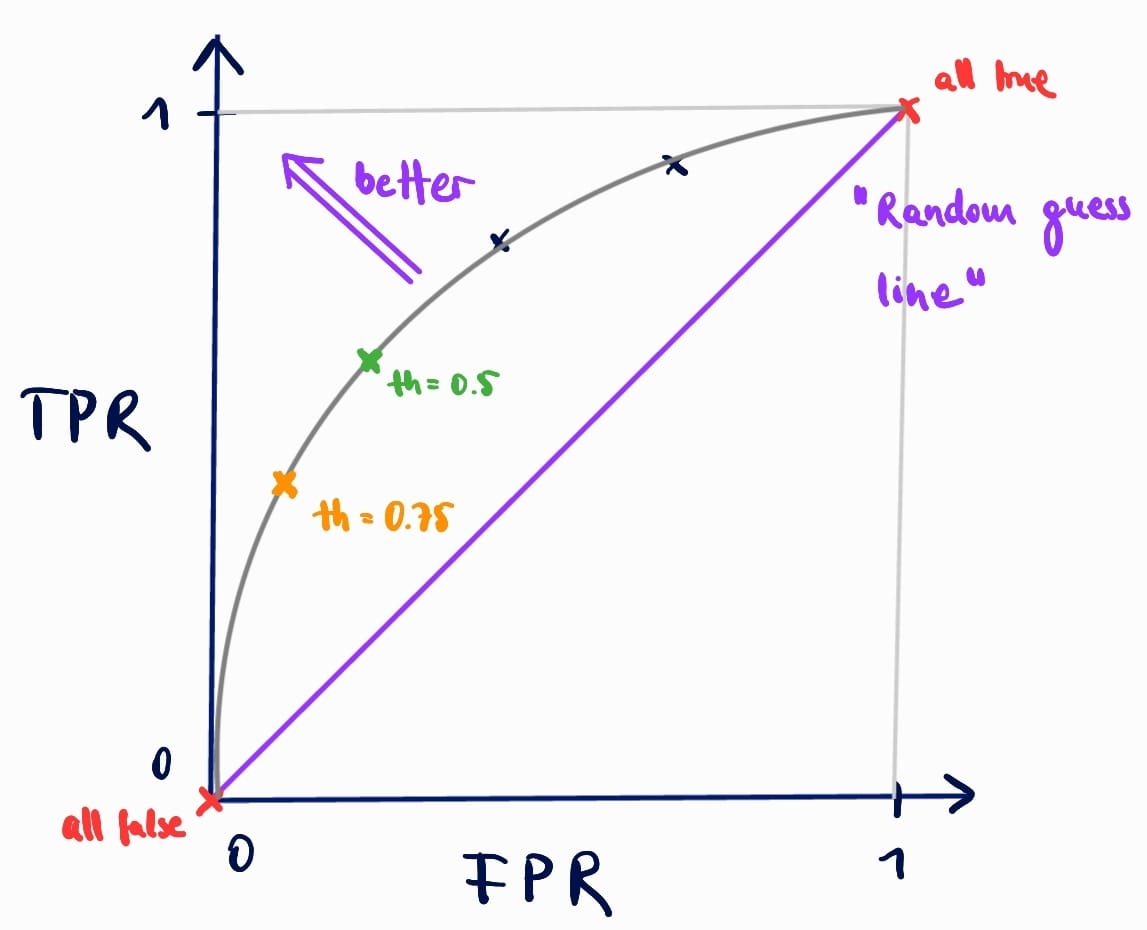
\includegraphics[width=\textwidth]{assets/sl/rocc__tpr_fpr.jpg}
  \end{subfigure}
  \vspace*{0.05\textwidth}
  \begin{subfigure}{0.5\textwidth}
    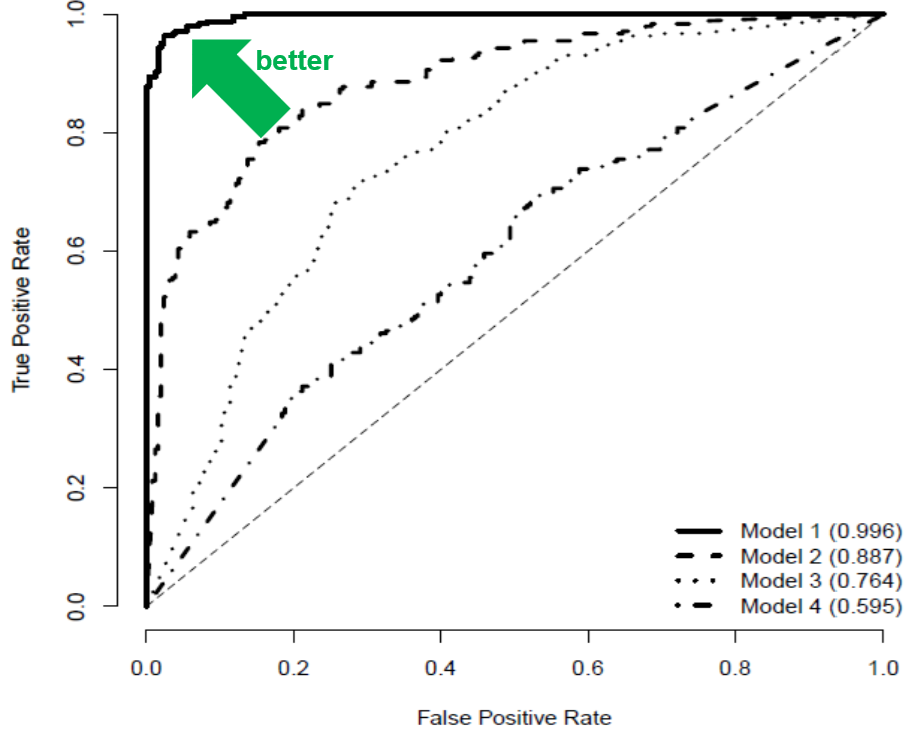
\includegraphics[width=\textwidth]{assets/sl/rocc__tpr_fpr_examples.png}
  \end{subfigure}

  \caption{Receiver Operating Characteristic Curve}
  \label{fig:7_ross_tpr_fpr}
\end{figure}

\begin{itemize}
  \item Define $q$ as the actually positive fraction, and $1-q$ the actually negative fraction
  \item With probability $p$ we now guess that an instance is positive, and with $1-p$ that an instance is negative\footnote{Following terms are only fractions, multiply with $N$ to get counts}
  \begin{align*}
    \implies TP &= pq & TN &= (1-p)(1-q)\\
    FP &= p(1-q) & FN &= (1-p)q
  \end{align*}
  \begin{align*}
    \implies TPR &= \frac{TP}{TP+FN} = \frac{pq}{pq + (1-p)q} = p\\ 
    TPR &= \frac{FP}{TN+FP} = \frac{p(1-q)}{(1-p)(1-q) + p(1-q)} = p
  \end{align*}
  \item This means: for random guessing as we described here, we have $TPR = p = FRP$ (where $q$ doesn't matter)
  \item To be better than this random guess, we need to maximize the \textbf{area under the curve (AUC)}\sidenote{Area Under The Curve}
  \begin{align*}
    ROC\ index = \sum_{i=2}^{|T|} & 
      \underbrace{\big(FPR(T[i]) - FPR(T[i-1])\big)}_{\text{steps }x\text{-axis}}\cdot 
      \underbrace{{\scriptstyle\frac{1}{2}}\big(TPR(T[i]) - TPR(T[i-1])\big)}_{\text{average height }y\text{-axis}} 
  \end{align*}
\end{itemize}

\begin{figure}[ht]
  \centering
  \begin{subfigure}{0.4\textwidth}
    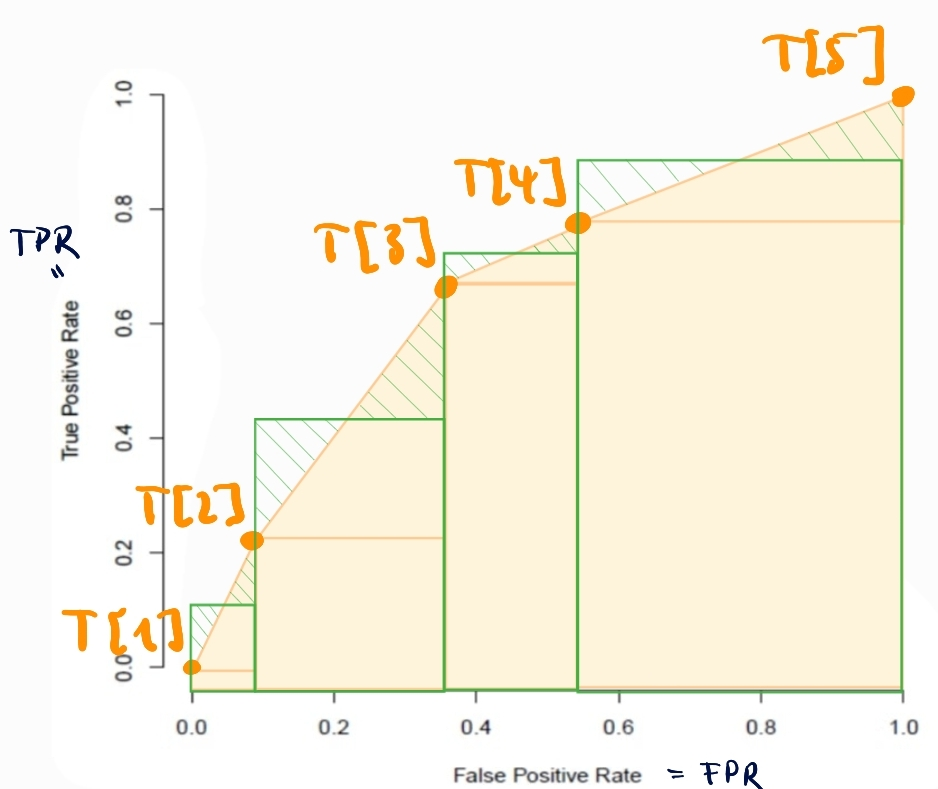
\includegraphics[width=\textwidth]{assets/sl/rocc__auc.jpg}
  \end{subfigure}

  \caption{Area Under the Curve (AUC)}
  \label{fig:7_ross_auc}
\end{figure}



